\documentclass{ltjsarticle}
\usepackage{graphics}
\begin{document}

\title{LilyPond-Bookによる楽譜入りドキュメント作成}
\author{haru}
\date{2024年4月1日}
\maketitle

\tableofcontents

\section{調}
\subsection{調とは}

調は、音楽を形作る重要な要素の1つで、楽曲の雰囲気などを司る。

主に長調と短調に分けられ、それぞれ12種類ずつある。  

\subsection{長調}

長調は比較的明るい印象を抱きやすい。

{%
\parindent 0pt
\noindent
\ifx\preLilyPondExample \undefined
\else
  \expandafter\preLilyPondExample
\fi
\def\lilypondbook{}%
\includegraphics{/mnt/c/Users/haru/working/zenn-test-2/test2/d2/lily-9b8b910c-1}%
% eof
%
\ifx\postLilyPondExample \undefined
\else
  \expandafter\postLilyPondExample
\fi
}

上記の調は最もスタンダードな「ハ長調」(C-dur, C Major)である。この他にも、

{%
\parindent 0pt
\noindent
\ifx\preLilyPondExample \undefined
\else
  \expandafter\preLilyPondExample
\fi
\def\lilypondbook{}%
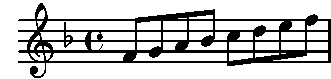
\includegraphics{/mnt/c/Users/haru/working/zenn-test-2/test2/5a/lily-d2bc86b8-1}%
% eof
%
\ifx\postLilyPondExample \undefined
\else
  \expandafter\postLilyPondExample
\fi
}

のような「ヘ長調」(F-dur, F Major)などがあるが、構成音の感覚は変化しない。これは短調についても言える。

\subsection{短調}

長調は1種類×12音=12種類であったが、短調は厳密には3種類あり、厳密に言うと3種類×12音=36種類存在することになる。  

\subsubsection{自然的短音階}

{%
\parindent 0pt
\noindent
\ifx\preLilyPondExample \undefined
\else
  \expandafter\preLilyPondExample
\fi
\def\lilypondbook{}%
\includegraphics{/mnt/c/Users/haru/working/zenn-test-2/test2/28/lily-6967f97f-1}%
% eof
%
\ifx\postLilyPondExample \undefined
\else
  \expandafter\postLilyPondExample
\fi
}

これはイ短調(A-moll, A minor)である。  
ハ長調とスタートとする音こそ異なるものの構成音が同じである。  
これらの調の関係を「平行調」という。  

\subsubsection{和声的短音階}

自然的短音階だと最後の音に上がる時に違和感が生じるが、それを改善した短音階。

{%
\parindent 0pt
\noindent
\ifx\preLilyPondExample \undefined
\else
  \expandafter\preLilyPondExample
\fi
\def\lilypondbook{}%
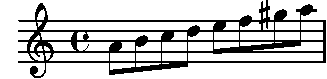
\includegraphics{/mnt/c/Users/haru/working/zenn-test-2/test2/d5/lily-fd893748-1}%
% eof
%
\ifx\postLilyPondExample \undefined
\else
  \expandafter\postLilyPondExample
\fi
}

\subsubsection{旋律的短音階}
和声的短音階の中東感を解決した短音階。\\
上行系と下行系が異なる。

{%
\parindent 0pt
\noindent
\ifx\preLilyPondExample \undefined
\else
  \expandafter\preLilyPondExample
\fi
\def\lilypondbook{}%
\includegraphics{/mnt/c/Users/haru/working/zenn-test-2/test2/fd/lily-d15d62a0-1}%
% eof
%
\ifx\postLilyPondExample \undefined
\else
  \expandafter\postLilyPondExample
\fi
}

\end{document}
